\section{Ideas \& Framework}
    This project proposes a computational–neuroscientific investigation of how humans solve constraint satisfaction problems (CSPs), such as Sudoku or map-coloring, through local, iterative reasoning processes analogous to \textbf{Belief Propagation (BP)} algorithms.  

    We hypothesize that individual behavioral patterns—and their associated neural dynamics—correspond to distinct \textbf{scheduling strategies} in BP, yielding characteristic convergence profiles observable in neural data.

    \subsection{Scientific Question}
    
%        \textbf{Central question:}  
%        \emph{Do human problem-solving behaviors and neural dynamics reflect asynchronous Belief Propagation (BP)–like processes, and can individual differences be explained as differences in message-passing scheduling policies?}
%
%        \textbf{Why important for neuroscience:}  
%        Understanding how humans iteratively combine local information to reach global solutions links computational-level theories (inference, constraint satisfaction) to neural mechanisms (distributed recurrent interactions). It provides a framework for interpreting reasoning as a form of message passing in neural circuits, bridging cognitive and circuit-level models of inference.
%        
%        \textbf{Broader insight:}  
%        This framework could ground high-level reasoning, attention, and expertise within a unified theory of distributed probabilistic computation, offering measurable indicators of algorithmic efficiency in both behavior and neural dynamics.


\subsubsection{Scientific Question 1: Local vs.\ Structured Inference}

Let \(G=(V,E)\) be a graph, \(X_i\) the target node to be reported, \(O\) the set of observed nodes, and \(H\setminus i\) the remaining unobserved nodes. We assume a standard pairwise graphical model:
\[
P(x_V)\propto \prod_{(u,v)\in E}\psi_{uv}(x_u,x_v)\prod_{u\in V}\phi_u(x_u).
\]

We contrast two hypotheses about human probabilistic inference.

\paragraph{H0: Local independent inference.}
Participants estimate \(X_i\) using only its locally observed neighbors \(O_i=N(i)\cap O\):
\[
P_{\mathrm{ind}}(x_i\mid x_O)
=
P(x_i\mid x_{O_i})
\propto
\phi_i(x_i)\prod_{j\in O_i}\psi_{ij}(x_i,x_j).
\]
Under this hypothesis, if the local observed neighborhood of \(X_i\) is held fixed, then changing distal structure or distal evidence should not affect the reported belief:
\[
P_{\mathrm{ind}}^{(A)}(x_i\mid x_O)=P_{\mathrm{ind}}^{(B)}(x_i\mid x_O).
\]

\paragraph{H1: Structured graph inference.}
Participants integrate over other unobserved variables, so the posterior of \(X_i\) depends on the broader graph structure:
\[
P_{\mathrm{struct}}(x_i\mid x_O)
=
\sum_{x_{H\setminus i}} P(x_i,x_{H\setminus i}\mid x_O).
\]
Equivalently,
\[
P_{\mathrm{struct}}(x_i\mid x_O)
\propto
\sum_{x_{H\setminus i}}
\left[
\prod_{(u,v)\in E}\psi_{uv}(x_u,x_v)\prod_{u\in V}\phi_u(x_u)
\right].
\]
Under this hypothesis, distal evidence can propagate through latent nodes, so even when the local observed neighborhood of \(X_i\) is unchanged, its posterior may differ across graph conditions:
\[
P_{\mathrm{struct}}^{(A)}(x_i\mid x_O)\neq P_{\mathrm{struct}}^{(B)}(x_i\mid x_O).
\]

\paragraph{Minimal chain example.}
For the three-node chain
\[
E - X_j - X_i,
\]
the two hypotheses make different predictions. Under local independent inference,
\[
P_{\mathrm{ind}}(x_i\mid E)=P(x_i),
\]
because \(X_i\) has no directly observed neighbor. Under structured inference,
\[
P_{\mathrm{struct}}(x_i\mid E)
\propto
\sum_{x_j} P(x_i\mid x_j)P(x_j\mid E),
\]
so the distal evidence at \(E\) affects the posterior of \(X_i\) via the hidden intermediate node \(X_j\).

        
        
     \subsection{Task design}
% Packages needed in preamble:
% \usepackage{tikz}
% \usetikzlibrary{positioning}
% \usepackage{subcaption} % optional, only if you want subfigure references elsewhere

% TikZ styles
\tikzset{
    latent/.style={circle, draw, thick, minimum size=8mm, inner sep=0pt},
    observed/.style={circle, draw, thick, fill=gray!25, minimum size=8mm, inner sep=0pt},
    target/.style={circle, draw, very thick, double, minimum size=8mm, inner sep=0pt}
}

\begin{figure}[ht]
\centering

% ---------------- Row 1 ----------------
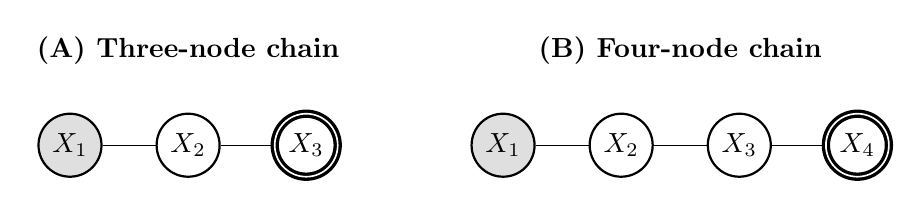
\begin{tikzpicture}[node distance=14mm and 14mm]

% ===== Panel A: 3-node chain =====
\begin{scope}[shift={(0,0)}]
    \node at (1.5,1.2) {\textbf{(A) Three-node chain}};
    \node[observed] (a1) at (0,0) {\(X_1\)};
    \node[latent]   (a2) at (1.5,0) {\(X_2\)};
    \node[target]   (a3) at (3,0) {\(X_3\)};
    \draw (a1) -- (a2) -- (a3);
\end{scope}

% ===== Panel B: 4-node chain =====
\begin{scope}[shift={(5.5,0)}]
    \node at (2.25,1.2) {\textbf{(B) Four-node chain}};
    \node[observed] (b1) at (0,0) {\(X_1\)};
    \node[latent]   (b2) at (1.5,0) {\(X_2\)};
    \node[latent]   (b3) at (3,0) {\(X_3\)};
    \node[target]   (b4) at (4.5,0) {\(X_4\)};
    \draw (b1) -- (b2) -- (b3) -- (b4);
\end{scope}

\end{tikzpicture}

\vspace{1em}

% ---------------- Row 2 ----------------
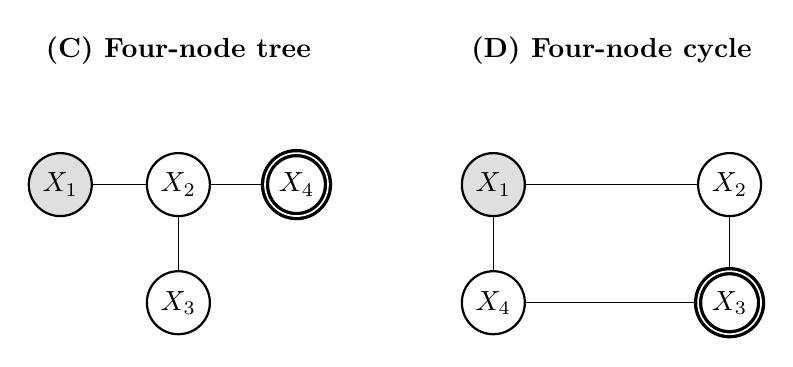
\begin{tikzpicture}[node distance=14mm and 14mm]

% ===== Panel C: 4-node tree =====
\begin{scope}[shift={(0,0)}]
    \node at (1.5,1.7) {\textbf{(C) Four-node tree}};
    \node[latent]   (c2) at (1.5,0) {\(X_2\)};
    \node[observed] (c1) at (0,0) {\(X_1\)};
    \node[latent]   (c3) at (1.5,-1.5) {\(X_3\)};
    \node[target]   (c4) at (3,0) {\(X_4\)};
    \draw (c1) -- (c2);
    \draw (c2) -- (c3);
    \draw (c2) -- (c4);
\end{scope}

% ===== Panel D: 4-node cycle =====
\begin{scope}[shift={(5.5,0)}]
    \node at (1.5,1.7) {\textbf{(D) Four-node cycle}};
    \node[observed] (d1) at (0,0) {\(X_1\)};
    \node[latent]   (d2) at (3,0) {\(X_2\)};
    \node[target]   (d3) at (3,-1.5) {\(X_3\)};
    \node[latent]   (d4) at (0,-1.5) {\(X_4\)};
    \draw (d1) -- (d2) -- (d3) -- (d4) -- (d1);
\end{scope}

\end{tikzpicture}

\caption{
Graphical models used in the experiment. Gray nodes are observed evidence nodes (\(X_1\); either hard or soft evidence), double-circle nodes are target nodes to be reported by participants, and single-circle nodes are latent unreported nodes.
}
\label{fig:graphical_models_four_panels}
\end{figure}


    \subsection{Related Work}
        Prior work connects statistical physics, information theory, and cognition through constraint satisfaction models (Mézard \& Mora, 2008).  
        Belief Propagation (BP) and related message-passing methods have explained efficient inference in large-scale optimization and neural-inspired algorithms.  
        In cognitive science, human reasoning has been modeled as probabilistic inference (Griffiths, Tenenbaum), but few studies have tested whether the \emph{dynamics} of human reasoning—its temporal evolution—match known algorithmic convergence profiles.  
        Neuroscientific frameworks like predictive coding and recurrent inference posit local error correction but have not mapped these precisely to algorithmic scheduling strategies.  
        \textbf{The gap:} Empirical linking of behavioral sequences, algorithmic update dynamics, and neural temporal patterns remains untested.

    \subsection{Theoretical Framework}
        \begin{itemize}
            \item \textbf{Core theory:} Humans solve structured reasoning problems through distributed, local message passing, akin to asynchronous BP on graphical models. Each attended variable update corresponds to a local message computation; scheduling (the order and timing of updates) determines efficiency and convergence, analogous to expertise.
            \item \textbf{Key predictions:}
                  \begin{itemize}
                      \item Behavioral sequences reveal implicit scheduling strategies matching algorithmic scheduling rules (e.g., conflict-driven, uncertainty-driven).
                      \item Convergence rate and stability in human problem solving mirror BP convergence profiles.
                      \item Neural dynamics (oscillatory coupling, activity stabilization) correlate with algorithmic convergence curves.
                      \item Experts show faster convergence and reduced oscillatory instability—signatures of optimized scheduling.
                  \end{itemize}
            \item \textbf{Level of analysis:} Cognitive (reasoning steps and attention dynamics) $\rightarrow$ algorithmic (scheduling and convergence) $\rightarrow$ dynamical/circuit-level (recurrent neural message passing).
        \end{itemize}
    
    \subsection{General Task Design}
        
        \paragraph{Paradigm}
            Participants solve simplified CSPs (e.g., 4×4 Sudoku, 5-region map-coloring).  
            Each variable (cell/region) is connected to constraints governing valid assignments.  
            Participants interact via mouse clicks or gaze, allowing tracking of the \textbf{sequence and timing of variable updates}.
            
            \begin{itemize}
                \item \textbf{Independent variables:} Constraint density (analogous to clause density $\alpha$); expertise level (novice vs. trained).
                \item \textbf{Dependent variables:} Sequence of attention/focus (scheduling traces), reaction times, corrections, solution time, accuracy.
            \end{itemize}
    
        \paragraph{Measurable Outcomes}
            \begin{itemize}
                \item \textbf{Behavioral:} Sequences of variable selection, reaction times, confidence, constraint violation rate.
                \item \textbf{Neural:} EEG/MEG oscillations, fMRI activity coupling, or ECoG dynamics during reasoning.
            \end{itemize}
    
    \subsection{Data Sources and Experimental Setup}
        \begin{itemize}
            \item \textbf{Behavioral datasets:} Newly collected CSP solving data (lab-based or online), high temporal resolution.
            \item \textbf{Neural recordings:} EEG/MEG for timing, fMRI for network topology, possible ECoG or calcium imaging in animal models.
            \item \textbf{Limitations:} Requires alignment between behavioral updates and neural signals; BP model parameterization depends on known graph connectivity.
        \end{itemize}
    
    \subsection{Computational Models and Analyses}
        
        \paragraph{Model Specification}
            \begin{itemize}
                \item \textbf{Candidate models:}
                      \begin{enumerate}
                          \item BP with different scheduling policies (random, sequential, conflict-driven, uncertainty-driven).
                          \item Human-derived scheduling BP (using observed behavioral order).
                          \item Null models: random search or heuristic solvers.
                      \end{enumerate}
                \item \textbf{Parameters:} Scheduling rule weights, damping coefficients (belief stability), convergence rate constants (fit to behavioral and neural time courses).
            \end{itemize}
        
        \paragraph{Model Comparison}
            \begin{itemize}
                \item Metrics: log-likelihood, BIC/AIC, cross-validation.
                \item Hierarchical comparison across participants to identify scheduling families.
            \end{itemize}

        \paragraph{Hypothesis Testing}
            \begin{itemize}
                \item \textbf{Null:} Human sequences arise from random or heuristic search.
                \item \textbf{Test:} BP with individualized scheduling fits better to timing, sequence, and convergence trajectories.
                \item \textbf{Robustness:} Bootstrap and permutation tests.
            \end{itemize}

        \paragraph{Neural Data Analyses}
            \begin{itemize}
                \item Encoding/decoding models linking neural patterns to BP message dynamics.
                \item Dimensionality reduction (PCA, GPFA) to identify latent convergence trajectories.
                \item Representational similarity between neural and algorithmic convergence curves (e.g., dynamic time warping).
            \end{itemize}
    
    \subsection{Evaluation Plan}
        \begin{itemize}
            \item \textbf{Behavioral:} Alignment between observed and modeled update order, correlation of convergence rates, recovery of scheduling parameters.
            \item \textbf{Neural:} Variance in neural activity explained by BP convergence, cross-correlation between neural stabilization and algorithmic energy minimization, similarity between neural and simulated belief trajectories.
            \item \textbf{Theory validation:} Consistent behavioral and neural evidence for BP-like convergence dynamics supports message-passing as a neural computation principle.
        \end{itemize}

\subsection{Next Steps and Open Questions}
    \begin{itemize}
        \item \textbf{Planned experiments:} Scale complexity/constraint density to test phase-transition effects; longitudinal training to observe evolving scheduling strategies.
        \item \textbf{Risks:} Neural activity may reflect other cognitive processes (e.g., WM, planning); data may admit multiple model fits.
        \item \textbf{Mitigations:} Diverse task types, replication, and strong model-comparison criteria.
        \item \textbf{Generalization:} Theory extends to other reasoning domains (planning, language comprehension) where distributed constraint satisfaction and message passing are central.
    \end{itemize}
    
    \textbf{Summary:}  
    This project operationalizes human reasoning as asynchronous Belief Propagation, tests its algorithmic traces in behavior, and maps its convergence dynamics to neural dynamics. By inferring each participant’s implicit scheduling policy, we aim to reveal how cognitive expertise and brain networks jointly implement distributed probabilistic inference.

\subsection{引言}
约束满足问题（Constraint Satisfaction Problems, CSPs）构成高阶认知的计算基石。从规划日常行程到推演复杂社会层级，人类大脑须持续协调变量间的相互约束，以达成全局一致的认知状态。然而，支撑这一过程的算法架构至今仍是争论焦点。经典符号主义认知理论主张，人类通过串行启发式搜索求解此类问题——一个包含赋值、冲突检测与回溯的离散阶梯式过程（Newell \& Simon, 1976）。源自概率计算与统计物理的新兴视角则提出，大脑可能运作如同分布式推断引擎，借助类似信念传播（Belief Propagation, BP）的并行消息传递算法，通过迭代一致化逼近边缘概率并收敛至解（Friston, 2010; Pegev \& Pouget, 2023）。这两种观点代表了理解神经计算语法的根本性分歧：推理究竟是一系列严密的逻辑运算，还是动力系统向能量极小值的逐渐收敛过程？

地图填色任务为解决这一争议提供了理想的实验范式。与深受语义先验干扰的语言推理不同，地图填色分离了约束满足的纯结构动力学，使研究者得以在受控条件下考察计算机制本身。更为关键的是，CSP 在计算复杂性上表现出由约束-变量比率控制的剧烈相变现象。正是在这一临界区域——问题虽可解但计算代价高昂——不同算法的特征差异才最为显著。串行搜索模型预测反应时间将呈现由回溯深度驱动的重尾分布；分布式推断模型则预测，在系统未陷入局部极小值的前提下，收敛时间与网络规模呈对数关系（Zdeborová \& Krzakala, 2016）。既往行为学研究多未能有效控制这一算法硬度参数，致使人类表现数据往往能被两类框架事后拟合，结论难以判定。

本研究提出一个统一的计算框架，旨在通过行为表型、跨任务迁移与神经动力学的三角互证来剖析这一机制。该框架的核心前提是：若大脑采用类 BP 机制，其"解"便不应仅是最终状态，而是对约束景观的一种鲁棒概率表征。据此，学习效应应当在具有拓扑同构性的地图间迁移——即局部消息传递结构保持不变——而非仅迁移抽象的启发式规则（如"优先填涂连接度最高的节点"）。这一区分至关重要：符号系统迁移的是产生式规则，而分布式系统迁移的是结构统计量。

对这两类模型的裁决还要求超越简单的激活映射，深入考察神经时间序列的几何特征。两种计算假说对神经状态轨迹提出了截然不同的预测。分布式推断过程意味着神经表征将呈现连续的、类梯度的演化，渐进逼近一致状态——这一过程可能映射为顶叶与前额叶皮层群体编码的逐渐锐化。相反，串行搜索蕴含着对应于决策节点与错误信号的离散突变式状态转换，极可能表现为与工作记忆更新相关的特定振荡爆发（如 theta-gamma 耦合）或重置信号。

通过将严谨的算法控制与高维神经解码相结合，本框架旨在超越"大脑即计算机"的简单隐喻，确定生物体在求解 NP 难问题时究竟依赖于对符号的精确句法操作，还是进化偏好了一种弛豫策略——即逻辑涌现于神经网络的动力学平衡过程之中。这一问题的解答不仅将厘清人类推理的架构边界，更将为设计具备灵活约束满足能力的神经形态系统提供理论基础。